\PassOptionsToPackage{unicode=true}{hyperref} % options for packages loaded elsewhere
\PassOptionsToPackage{hyphens}{url}
%
\documentclass[]{article}
\usepackage{lmodern}
\usepackage{amssymb,amsmath}
\usepackage{ifxetex,ifluatex}
\usepackage{fixltx2e} % provides \textsubscript
\ifnum 0\ifxetex 1\fi\ifluatex 1\fi=0 % if pdftex
  \usepackage[T1]{fontenc}
  \usepackage[utf8]{inputenc}
  \usepackage{textcomp} % provides euro and other symbols
\else % if luatex or xelatex
  \usepackage{unicode-math}
  \defaultfontfeatures{Ligatures=TeX,Scale=MatchLowercase}
\fi
% use upquote if available, for straight quotes in verbatim environments
\IfFileExists{upquote.sty}{\usepackage{upquote}}{}
% use microtype if available
\IfFileExists{microtype.sty}{%
\usepackage[]{microtype}
\UseMicrotypeSet[protrusion]{basicmath} % disable protrusion for tt fonts
}{}
\IfFileExists{parskip.sty}{%
\usepackage{parskip}
}{% else
\setlength{\parindent}{0pt}
\setlength{\parskip}{6pt plus 2pt minus 1pt}
}
\usepackage{hyperref}
\hypersetup{
            pdftitle={Assignment 6: GLMs week 1 (t-test and ANOVA)},
            pdfauthor={Rachel Gonsenhauser},
            pdfborder={0 0 0},
            breaklinks=true}
\urlstyle{same}  % don't use monospace font for urls
\usepackage[margin=2.54cm]{geometry}
\usepackage{color}
\usepackage{fancyvrb}
\newcommand{\VerbBar}{|}
\newcommand{\VERB}{\Verb[commandchars=\\\{\}]}
\DefineVerbatimEnvironment{Highlighting}{Verbatim}{commandchars=\\\{\}}
% Add ',fontsize=\small' for more characters per line
\usepackage{framed}
\definecolor{shadecolor}{RGB}{248,248,248}
\newenvironment{Shaded}{\begin{snugshade}}{\end{snugshade}}
\newcommand{\AlertTok}[1]{\textcolor[rgb]{0.94,0.16,0.16}{#1}}
\newcommand{\AnnotationTok}[1]{\textcolor[rgb]{0.56,0.35,0.01}{\textbf{\textit{#1}}}}
\newcommand{\AttributeTok}[1]{\textcolor[rgb]{0.77,0.63,0.00}{#1}}
\newcommand{\BaseNTok}[1]{\textcolor[rgb]{0.00,0.00,0.81}{#1}}
\newcommand{\BuiltInTok}[1]{#1}
\newcommand{\CharTok}[1]{\textcolor[rgb]{0.31,0.60,0.02}{#1}}
\newcommand{\CommentTok}[1]{\textcolor[rgb]{0.56,0.35,0.01}{\textit{#1}}}
\newcommand{\CommentVarTok}[1]{\textcolor[rgb]{0.56,0.35,0.01}{\textbf{\textit{#1}}}}
\newcommand{\ConstantTok}[1]{\textcolor[rgb]{0.00,0.00,0.00}{#1}}
\newcommand{\ControlFlowTok}[1]{\textcolor[rgb]{0.13,0.29,0.53}{\textbf{#1}}}
\newcommand{\DataTypeTok}[1]{\textcolor[rgb]{0.13,0.29,0.53}{#1}}
\newcommand{\DecValTok}[1]{\textcolor[rgb]{0.00,0.00,0.81}{#1}}
\newcommand{\DocumentationTok}[1]{\textcolor[rgb]{0.56,0.35,0.01}{\textbf{\textit{#1}}}}
\newcommand{\ErrorTok}[1]{\textcolor[rgb]{0.64,0.00,0.00}{\textbf{#1}}}
\newcommand{\ExtensionTok}[1]{#1}
\newcommand{\FloatTok}[1]{\textcolor[rgb]{0.00,0.00,0.81}{#1}}
\newcommand{\FunctionTok}[1]{\textcolor[rgb]{0.00,0.00,0.00}{#1}}
\newcommand{\ImportTok}[1]{#1}
\newcommand{\InformationTok}[1]{\textcolor[rgb]{0.56,0.35,0.01}{\textbf{\textit{#1}}}}
\newcommand{\KeywordTok}[1]{\textcolor[rgb]{0.13,0.29,0.53}{\textbf{#1}}}
\newcommand{\NormalTok}[1]{#1}
\newcommand{\OperatorTok}[1]{\textcolor[rgb]{0.81,0.36,0.00}{\textbf{#1}}}
\newcommand{\OtherTok}[1]{\textcolor[rgb]{0.56,0.35,0.01}{#1}}
\newcommand{\PreprocessorTok}[1]{\textcolor[rgb]{0.56,0.35,0.01}{\textit{#1}}}
\newcommand{\RegionMarkerTok}[1]{#1}
\newcommand{\SpecialCharTok}[1]{\textcolor[rgb]{0.00,0.00,0.00}{#1}}
\newcommand{\SpecialStringTok}[1]{\textcolor[rgb]{0.31,0.60,0.02}{#1}}
\newcommand{\StringTok}[1]{\textcolor[rgb]{0.31,0.60,0.02}{#1}}
\newcommand{\VariableTok}[1]{\textcolor[rgb]{0.00,0.00,0.00}{#1}}
\newcommand{\VerbatimStringTok}[1]{\textcolor[rgb]{0.31,0.60,0.02}{#1}}
\newcommand{\WarningTok}[1]{\textcolor[rgb]{0.56,0.35,0.01}{\textbf{\textit{#1}}}}
\usepackage{graphicx,grffile}
\makeatletter
\def\maxwidth{\ifdim\Gin@nat@width>\linewidth\linewidth\else\Gin@nat@width\fi}
\def\maxheight{\ifdim\Gin@nat@height>\textheight\textheight\else\Gin@nat@height\fi}
\makeatother
% Scale images if necessary, so that they will not overflow the page
% margins by default, and it is still possible to overwrite the defaults
% using explicit options in \includegraphics[width, height, ...]{}
\setkeys{Gin}{width=\maxwidth,height=\maxheight,keepaspectratio}
\setlength{\emergencystretch}{3em}  % prevent overfull lines
\providecommand{\tightlist}{%
  \setlength{\itemsep}{0pt}\setlength{\parskip}{0pt}}
\setcounter{secnumdepth}{0}
% Redefines (sub)paragraphs to behave more like sections
\ifx\paragraph\undefined\else
\let\oldparagraph\paragraph
\renewcommand{\paragraph}[1]{\oldparagraph{#1}\mbox{}}
\fi
\ifx\subparagraph\undefined\else
\let\oldsubparagraph\subparagraph
\renewcommand{\subparagraph}[1]{\oldsubparagraph{#1}\mbox{}}
\fi

% set default figure placement to htbp
\makeatletter
\def\fps@figure{htbp}
\makeatother


\title{Assignment 6: GLMs week 1 (t-test and ANOVA)}
\author{Rachel Gonsenhauser}
\date{}

\begin{document}
\maketitle

\hypertarget{overview}{%
\subsection{OVERVIEW}\label{overview}}

This exercise accompanies the lessons in Environmental Data Analytics on
t-tests and ANOVAs.

\hypertarget{directions}{%
\subsection{Directions}\label{directions}}

\begin{enumerate}
\def\labelenumi{\arabic{enumi}.}
\tightlist
\item
  Change ``Student Name'' on line 3 (above) with your name.
\item
  Work through the steps, \textbf{creating code and output} that fulfill
  each instruction.
\item
  Be sure to \textbf{answer the questions} in this assignment document.
\item
  When you have completed the assignment, \textbf{Knit} the text and
  code into a single PDF file.
\item
  After Knitting, submit the completed exercise (PDF file) to the
  dropbox in Sakai. Add your last name into the file name (e.g.,
  ``Salk\_A06\_GLMs\_Week1.Rmd'') prior to submission.
\end{enumerate}

The completed exercise is due on Tuesday, February 18 at 1:00 pm.

\hypertarget{set-up-your-session}{%
\subsection{Set up your session}\label{set-up-your-session}}

\begin{enumerate}
\def\labelenumi{\arabic{enumi}.}
\item
  Check your working directory, load the \texttt{tidyverse},
  \texttt{cowplot}, and \texttt{agricolae} packages, and import the
  NTL-LTER\_Lake\_Nutrients\_PeterPaul\_Processed.csv dataset.
\item
  Change the date column to a date format. Call up \texttt{head} of this
  column to verify.
\end{enumerate}

\begin{Shaded}
\begin{Highlighting}[]
\CommentTok{#1}
\KeywordTok{getwd}\NormalTok{()}
\end{Highlighting}
\end{Shaded}

\begin{verbatim}
## [1] "/Users/rachelgonsenhauser/Documents/Environmental_Data_Analytics_2020"
\end{verbatim}

\begin{Shaded}
\begin{Highlighting}[]
\KeywordTok{library}\NormalTok{(tidyverse)}
\KeywordTok{library}\NormalTok{(cowplot)}
\CommentTok{#install.packages("agricolae")}
\KeywordTok{library}\NormalTok{(agricolae)}
\NormalTok{PeterPaul.Processed <-}
\StringTok{  }\KeywordTok{read.csv}\NormalTok{(}\StringTok{"./Data/Processed/NTL-LTER_Lake_Nutrients_PeterPaul_Processed.csv"}\NormalTok{)}

\CommentTok{#2}
\KeywordTok{class}\NormalTok{(PeterPaul.Processed}\OperatorTok{$}\NormalTok{sampledate)}
\end{Highlighting}
\end{Shaded}

\begin{verbatim}
## [1] "factor"
\end{verbatim}

\begin{Shaded}
\begin{Highlighting}[]
\NormalTok{PeterPaul.Processed}\OperatorTok{$}\NormalTok{sampledate <-}\StringTok{ }\KeywordTok{as.Date}\NormalTok{(}
\NormalTok{  PeterPaul.Processed}\OperatorTok{$}\NormalTok{sampledate, }\DataTypeTok{format =} \StringTok{"%Y-%m-%d"}\NormalTok{)}
\KeywordTok{class}\NormalTok{(PeterPaul.Processed}\OperatorTok{$}\NormalTok{sampledate)}
\end{Highlighting}
\end{Shaded}

\begin{verbatim}
## [1] "Date"
\end{verbatim}

\begin{Shaded}
\begin{Highlighting}[]
\KeywordTok{head}\NormalTok{(PeterPaul.Processed)}
\end{Highlighting}
\end{Shaded}

\begin{verbatim}
##   lakeid  lakename year4 daynum month sampledate depth_id depth tn_ug tp_ug
## 1      L Paul Lake  1991    140     5 1991-05-20        1  0.00   538    25
## 2      L Paul Lake  1991    140     5 1991-05-20        2  0.85   285    14
## 3      L Paul Lake  1991    140     5 1991-05-20        3  1.75   399    14
## 4      L Paul Lake  1991    140     5 1991-05-20        4  3.00   453    14
## 5      L Paul Lake  1991    140     5 1991-05-20        5  4.00   363    13
## 6      L Paul Lake  1991    140     5 1991-05-20        6  6.00   583    37
##   nh34 no23 po4 comments
## 1   NA   NA  NA       NA
## 2   NA   NA  NA       NA
## 3   NA   NA  NA       NA
## 4   NA   NA  NA       NA
## 5   NA   NA  NA       NA
## 6   NA   NA  NA       NA
\end{verbatim}

\hypertarget{wrangle-your-data}{%
\subsection{Wrangle your data}\label{wrangle-your-data}}

\begin{enumerate}
\def\labelenumi{\arabic{enumi}.}
\setcounter{enumi}{2}
\tightlist
\item
  Wrangle your dataset so that it contains only surface depths and only
  the years 1993-1996, inclusive. Set month as a factor.
\end{enumerate}

\begin{Shaded}
\begin{Highlighting}[]
\NormalTok{PeterPaul.Wrangled <-}\StringTok{ }\KeywordTok{filter}\NormalTok{(PeterPaul.Processed, depth }\OperatorTok{==}\StringTok{ }\DecValTok{0}\NormalTok{) }
\NormalTok{PeterPaul.Wrangled <-}\StringTok{ }\KeywordTok{filter}\NormalTok{(PeterPaul.Wrangled, year4 }\OperatorTok\StringTok{ }\KeywordTok{c}\NormalTok{(}\DecValTok{1993}\OperatorTok{:}\DecValTok{1996}\NormalTok{))}
\NormalTok{  PeterPaul.Wrangled}\OperatorTok{$}\NormalTok{month <-}\StringTok{ }\KeywordTok{as.factor}\NormalTok{(PeterPaul.Wrangled}\OperatorTok{$}\NormalTok{month)}
\KeywordTok{class}\NormalTok{(PeterPaul.Wrangled}\OperatorTok{$}\NormalTok{month)}
\end{Highlighting}
\end{Shaded}

\begin{verbatim}
## [1] "factor"
\end{verbatim}

\hypertarget{analysis}{%
\subsection{Analysis}\label{analysis}}

Peter Lake was manipulated with additions of nitrogen and phosphorus
over the years 1993-1996 in an effort to assess the impacts of
eutrophication in lakes. You are tasked with finding out if nutrients
are significantly higher in Peter Lake than Paul Lake, and if these
potential differences in nutrients vary seasonally (use month as a
factor to represent seasonality). Run two separate tests for TN and TP.

\begin{enumerate}
\def\labelenumi{\arabic{enumi}.}
\setcounter{enumi}{3}
\tightlist
\item
  Which application of the GLM will you use (t-test, one-way ANOVA,
  two-way ANOVA with main effects, or two-way ANOVA with interaction
  effects)? Justify your choice.
\end{enumerate}

\begin{quote}
Answer: I chose to use a two-way ANOVA because in this case the
explanatory variable (total nitrogen or total phosphorous) is continuous
and the two explanatory variables (lake and month) are categorical.
Specifically, I ran a two-way ANOVA with interaction effects to test
whether there was an interaction between the explanatory variables on
total nitrogen or phosphorous values.
\end{quote}

\begin{enumerate}
\def\labelenumi{\arabic{enumi}.}
\setcounter{enumi}{4}
\item
  Run your test for TN. Include examination of groupings and consider
  interaction effects, if relevant.
\item
  Run your test for TP. Include examination of groupings and consider
  interaction effects, if relevant.
\end{enumerate}

\begin{Shaded}
\begin{Highlighting}[]
\CommentTok{#5 }
\NormalTok{PeterPaul.TN.anova}\FloatTok{.2}\NormalTok{way <-}\StringTok{ }
\StringTok{  }\KeywordTok{aov}\NormalTok{(}\DataTypeTok{data =}\NormalTok{ PeterPaul.Wrangled, tn_ug }\OperatorTok{~}\StringTok{ }\NormalTok{lakename }\OperatorTok{*}\StringTok{ }\NormalTok{month)}
\KeywordTok{summary}\NormalTok{(PeterPaul.TN.anova}\FloatTok{.2}\NormalTok{way)}
\end{Highlighting}
\end{Shaded}

\begin{verbatim}
##                Df  Sum Sq Mean Sq F value   Pr(>F)    
## lakename        1 2468595 2468595  36.414 2.91e-08 ***
## month           4  459542  114885   1.695    0.157    
## lakename:month  4  288272   72068   1.063    0.379    
## Residuals      97 6575834   67792                     
## ---
## Signif. codes:  0 '***' 0.001 '**' 0.01 '*' 0.05 '.' 0.1 ' ' 1
## 23 observations deleted due to missingness
\end{verbatim}

\begin{Shaded}
\begin{Highlighting}[]
\KeywordTok{plot}\NormalTok{(PeterPaul.TN.anova}\FloatTok{.2}\NormalTok{way)}
\end{Highlighting}
\end{Shaded}

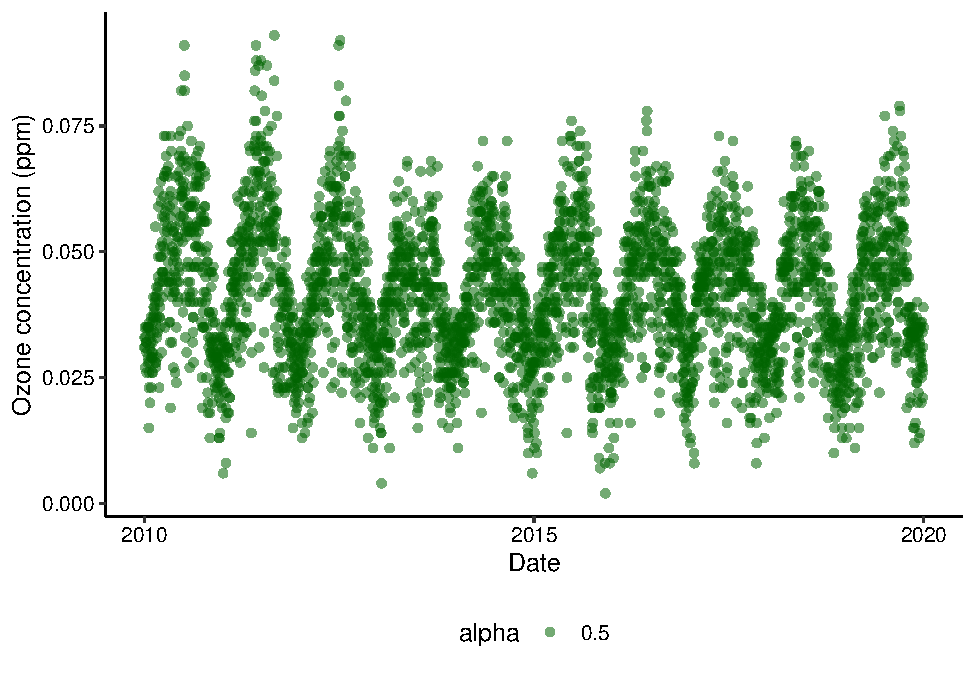
\includegraphics{A06_GLMs_Week1_files/figure-latex/unnamed-chunk-3-1.pdf}
\includegraphics{A06_GLMs_Week1_files/figure-latex/unnamed-chunk-3-2.pdf}
\includegraphics{A06_GLMs_Week1_files/figure-latex/unnamed-chunk-3-3.pdf}
\includegraphics{A06_GLMs_Week1_files/figure-latex/unnamed-chunk-3-4.pdf}

\begin{Shaded}
\begin{Highlighting}[]
\KeywordTok{TukeyHSD}\NormalTok{(PeterPaul.TN.anova}\FloatTok{.2}\NormalTok{way)}
\end{Highlighting}
\end{Shaded}

\begin{verbatim}
##   Tukey multiple comparisons of means
##     95% family-wise confidence level
## 
## Fit: aov(formula = tn_ug ~ lakename * month, data = PeterPaul.Wrangled)
## 
## $lakename
##                         diff      lwr      upr p adj
## Peter Lake-Paul Lake 303.796 203.8773 403.7146     0
## 
## $month
##          diff       lwr      upr     p adj
## 6-5 132.58168 -104.4173 369.5807 0.5296645
## 7-5 196.50011  -47.8276 440.8278 0.1755245
## 8-5 208.77984  -32.7942 450.3539 0.1234174
## 9-5 160.08048 -220.7887 540.9497 0.7692917
## 7-6  63.91843 -123.8978 251.7346 0.8780820
## 8-6  76.19815 -108.0216 260.4179 0.7795574
## 9-6  27.49879 -319.8343 374.8318 0.9994702
## 8-7  12.27972 -181.2775 205.8370 0.9997797
## 9-7 -36.41964 -388.7941 315.9548 0.9984863
## 9-8 -48.69936 -399.1701 301.7714 0.9952106
## 
## $`lakename:month`
##                                 diff         lwr       upr     p adj
## Peter Lake:5-Paul Lake:5    84.42736 -384.695091 553.54981 0.9998802
## Paul Lake:6-Paul Lake:5     23.61297 -376.795278 424.02122 1.0000000
## Peter Lake:6-Paul Lake:5   308.53119  -95.128061 712.19044 0.2949521
## Paul Lake:7-Paul Lake:5     53.12257 -358.325034 464.57018 0.9999929
## Peter Lake:7-Paul Lake:5   409.37327   -6.794730 825.54127 0.0577843
## Paul Lake:8-Paul Lake:5     35.99664 -375.450962 447.44425 0.9999998
## Peter Lake:8-Paul Lake:5   445.47177   38.159418 852.78411 0.0206524
## Paul Lake:9-Paul Lake:5    105.82450 -490.419726 702.06873 0.9998933
## Peter Lake:9-Paul Lake:5   249.95650 -438.527028 938.44003 0.9743614
## Paul Lake:6-Peter Lake:5   -60.81439 -439.493476 317.86470 0.9999541
## Peter Lake:6-Peter Lake:5  224.10383 -158.011173 606.21883 0.6694487
## Paul Lake:7-Peter Lake:5   -31.30479 -421.638257 359.02869 0.9999999
## Peter Lake:7-Peter Lake:5  324.94591  -70.360160 720.25198 0.2042224
## Paul Lake:8-Peter Lake:5   -48.43071 -438.764185 341.90276 0.9999950
## Peter Lake:8-Peter Lake:5  361.04441  -24.927657 747.01648 0.0870846
## Paul Lake:9-Peter Lake:5    21.39714 -560.477640 603.27193 1.0000000
## Peter Lake:9-Peter Lake:5  165.52914 -510.548261 841.60655 0.9985431
## Peter Lake:6-Paul Lake:6   284.91822   -8.787028 578.62346 0.0650344
## Paul Lake:7-Paul Lake:6     29.50960 -274.811140 333.83034 0.9999994
## Peter Lake:7-Paul Lake:6   385.76030   75.087182 696.43342 0.0043241
## Paul Lake:8-Paul Lake:6     12.38367 -291.937068 316.70441 1.0000000
## Peter Lake:8-Paul Lake:6   421.85880  123.152702 720.56489 0.0005774
## Paul Lake:9-Paul Lake:6     82.21153 -445.831232 610.25429 0.9999647
## Peter Lake:9-Paul Lake:6   226.34353 -403.998878 856.68594 0.9761624
## Paul Lake:7-Peter Lake:6  -255.40862 -563.994320  53.17709 0.1964898
## Peter Lake:7-Peter Lake:6  100.84208 -214.009961 415.69412 0.9891274
## Paul Lake:8-Peter Lake:6  -272.53454 -581.120248  36.05116 0.1316086
## Peter Lake:8-Peter Lake:6  136.94058 -166.109506 439.99066 0.9029804
## Paul Lake:9-Peter Lake:6  -202.70669 -733.218875 327.80550 0.9642843
## Peter Lake:9-Peter Lake:6  -58.57469 -690.987190 573.83782 0.9999996
## Peter Lake:7-Paul Lake:7   356.25070   31.473618 681.02778 0.0200027
## Paul Lake:8-Paul Lake:7    -17.12593 -335.831873 301.58002 1.0000000
## Peter Lake:8-Paul Lake:7   392.34920   79.000035 705.69836 0.0038467
## Paul Lake:9-Paul Lake:7     52.70193 -483.760115 589.16397 0.9999994
## Peter Lake:9-Paul Lake:7   196.83393 -440.577960 834.24582 0.9916222
## Paul Lake:8-Peter Lake:7  -373.37663 -698.153706 -48.59955 0.0116944
## Peter Lake:8-Peter Lake:7   36.09850 -283.423597 355.62059 0.9999978
## Paul Lake:9-Peter Lake:7  -303.54877 -843.639684 236.54215 0.7209271
## Peter Lake:9-Peter Lake:7 -159.41677 -799.885807 481.05227 0.9983429
## Peter Lake:8-Paul Lake:8   409.47512   96.125963 722.82428 0.0020552
## Paul Lake:9-Paul Lake:8     69.82786 -466.634186 606.28990 0.9999924
## Peter Lake:9-Paul Lake:8   213.95986 -423.452032 851.37175 0.9849047
## Paul Lake:9-Peter Lake:8  -339.64727 -872.944314 193.64978 0.5579223
## Peter Lake:9-Peter Lake:8 -195.51527 -830.265716 439.23518 0.9917740
## Peter Lake:9-Paul Lake:9   144.13200 -625.615985 913.87999 0.9998333
\end{verbatim}

\begin{Shaded}
\begin{Highlighting}[]
\NormalTok{TN.groupings <-}\StringTok{ }\KeywordTok{HSD.test}\NormalTok{(PeterPaul.TN.anova}\FloatTok{.2}\NormalTok{way, }
                         \StringTok{"lakename"}\NormalTok{, }\DataTypeTok{group =} \OtherTok{TRUE}\NormalTok{)}
\NormalTok{TN.groupings}
\end{Highlighting}
\end{Shaded}

\begin{verbatim}
## $statistics
##   MSerror Df     Mean       CV
##   67792.1 97 487.4077 53.41917
## 
## $parameters
##    test   name.t ntr StudentizedRange alpha
##   Tukey lakename   2         2.806822  0.05
## 
## $means
##               tn_ug      std  r     Min      Max      Q25     Q50      Q75
## Paul Lake  336.9293 100.2745 54  45.670  557.812 284.0107 344.243 411.5165
## Peter Lake 640.7253 361.3738 53 312.133 2048.151 448.0490 571.092 692.4860
## 
## $comparison
## NULL
## 
## $groups
##               tn_ug groups
## Peter Lake 640.7253      a
## Paul Lake  336.9293      b
## 
## attr(,"class")
## [1] "group"
\end{verbatim}

\begin{quote}
Total nitrogen differs significantly across the two lakes but does not
differ significantly seasonally (two-way ANOVA with interaction effects,
F1,4,4: 36.41, p\textless{}0.0001). Additionally, there is not a
sigificant interaction effect between lake and month on total nitrogen.
\end{quote}

\begin{Shaded}
\begin{Highlighting}[]
\CommentTok{#6}
\NormalTok{PeterPaul.TP.anova}\FloatTok{.2}\NormalTok{way <-}\StringTok{ }\KeywordTok{aov}\NormalTok{(}\DataTypeTok{data =}\NormalTok{ PeterPaul.Wrangled, tp_ug }\OperatorTok{~}\StringTok{ }\NormalTok{lakename }\OperatorTok{*}\StringTok{ }\NormalTok{month)}
\KeywordTok{summary}\NormalTok{(PeterPaul.TP.anova}\FloatTok{.2}\NormalTok{way)}
\end{Highlighting}
\end{Shaded}

\begin{verbatim}
##                 Df Sum Sq Mean Sq F value Pr(>F)    
## lakename         1  10228   10228  98.914 <2e-16 ***
## month            4    813     203   1.965 0.1043    
## lakename:month   4   1014     254   2.452 0.0496 *  
## Residuals      119  12305     103                   
## ---
## Signif. codes:  0 '***' 0.001 '**' 0.01 '*' 0.05 '.' 0.1 ' ' 1
## 1 observation deleted due to missingness
\end{verbatim}

\begin{Shaded}
\begin{Highlighting}[]
\KeywordTok{plot}\NormalTok{(PeterPaul.TP.anova}\FloatTok{.2}\NormalTok{way)}
\end{Highlighting}
\end{Shaded}

\includegraphics{A06_GLMs_Week1_files/figure-latex/unnamed-chunk-4-1.pdf}
\includegraphics{A06_GLMs_Week1_files/figure-latex/unnamed-chunk-4-2.pdf}
\includegraphics{A06_GLMs_Week1_files/figure-latex/unnamed-chunk-4-3.pdf}
\includegraphics{A06_GLMs_Week1_files/figure-latex/unnamed-chunk-4-4.pdf}

\begin{Shaded}
\begin{Highlighting}[]
\KeywordTok{TukeyHSD}\NormalTok{(PeterPaul.TP.anova}\FloatTok{.2}\NormalTok{way)}
\end{Highlighting}
\end{Shaded}

\begin{verbatim}
##   Tukey multiple comparisons of means
##     95% family-wise confidence level
## 
## Fit: aov(formula = tp_ug ~ lakename * month, data = PeterPaul.Wrangled)
## 
## $lakename
##                          diff      lwr      upr p adj
## Peter Lake-Paul Lake 17.80939 14.26365 21.35513     0
## 
## $month
##           diff         lwr       upr     p adj
## 6-5  6.3451786  -2.8038335 15.494191 0.3119085
## 7-5  8.8661326  -0.2828796 18.015145 0.0622967
## 8-5  4.8191843  -4.2626118 13.900980 0.5839528
## 9-5  5.4951391  -6.7194172 17.709695 0.7243206
## 7-6  2.5209540  -4.2125367  9.254445 0.8376355
## 8-6 -1.5259943  -8.1678685  5.115880 0.9688094
## 9-6 -0.8500395 -11.3776631  9.677584 0.9994372
## 8-7 -4.0469483 -10.6888225  2.594926 0.4453729
## 9-7 -3.3709935 -13.8986170  7.156630 0.9012092
## 9-8  0.6759548  -9.7933076 11.145217 0.9997679
## 
## $`lakename:month`
##                                  diff         lwr         upr     p adj
## Peter Lake:5-Paul Lake:5    4.3135714 -13.9293175  22.5564604 0.9989515
## Paul Lake:6-Paul Lake:5    -0.9178824 -16.4886641  14.6528993 1.0000000
## Peter Lake:6-Paul Lake:5   16.8838889   1.4263507  32.3414270 0.0206973
## Paul Lake:7-Paul Lake:5    -1.7271111 -17.1846493  13.7304270 0.9999981
## Peter Lake:7-Paul Lake:5   22.9304706   7.3596889  38.5012523 0.0002415
## Paul Lake:8-Paul Lake:5    -2.0872222 -17.5447604  13.3703159 0.9999902
## Peter Lake:8-Paul Lake:5   15.0200000  -0.3355071  30.3755071 0.0607728
## Paul Lake:9-Paul Lake:5    -0.7380000 -20.5935673  19.1175673 1.0000000
## Peter Lake:9-Paul Lake:5   14.7452500  -6.4208558  35.9113558 0.4316694
## Paul Lake:6-Peter Lake:5   -5.2314538 -19.9572479   9.4943403 0.9787107
## Peter Lake:6-Peter Lake:5  12.5703175  -2.0356832  27.1763181 0.1571717
## Paul Lake:7-Peter Lake:5   -6.0406825 -20.6466832   8.5653181 0.9437275
## Peter Lake:7-Peter Lake:5  18.6168992   3.8911050  33.3426933 0.0032014
## Paul Lake:8-Peter Lake:5   -6.4007937 -21.0067943   8.2052070 0.9208652
## Peter Lake:8-Peter Lake:5  10.7064286  -3.7915495  25.2044066 0.3464892
## Paul Lake:9-Peter Lake:5   -5.0515714 -24.2516579  14.1485150 0.9975850
## Peter Lake:9-Peter Lake:5  10.4316786 -10.1207861  30.9841433 0.8273658
## Peter Lake:6-Paul Lake:6   17.8017712   6.7120688  28.8914737 0.0000401
## Paul Lake:7-Paul Lake:6    -0.8092288 -11.8989312  10.2804737 1.0000000
## Peter Lake:7-Paul Lake:6   23.8483529  12.6013419  35.0953640 0.0000000
## Paul Lake:8-Paul Lake:6    -1.1693399 -12.2590423   9.9203626 0.9999989
## Peter Lake:8-Paul Lake:6   15.9378824   4.9908457  26.8849190 0.0003006
## Paul Lake:9-Paul Lake:6     0.1798824 -16.5021309  16.8618956 1.0000000
## Peter Lake:9-Paul Lake:6   15.6631324  -2.5591082  33.8853729 0.1584032
## Paul Lake:7-Peter Lake:6  -18.6110000 -29.5411300  -7.6808700 0.0000101
## Peter Lake:7-Peter Lake:6   6.0465817  -5.0431207  17.1362841 0.7595330
## Paul Lake:8-Peter Lake:6  -18.9711111 -29.9012412  -8.0409811 0.0000062
## Peter Lake:8-Peter Lake:6  -1.8638889 -12.6492426   8.9214648 0.9999197
## Paul Lake:9-Peter Lake:6  -17.6218889 -34.1982518  -1.0455259 0.0276305
## Peter Lake:9-Peter Lake:6  -2.1386389 -20.2642090  15.9869312 0.9999970
## Peter Lake:7-Paul Lake:7   24.6575817  13.5678793  35.7472841 0.0000000
## Paul Lake:8-Paul Lake:7    -0.3601111 -11.2902412  10.5700189 1.0000000
## Peter Lake:8-Paul Lake:7   16.7471111   5.9617574  27.5324648 0.0000827
## Paul Lake:9-Paul Lake:7     0.9891111 -15.5872518  17.5654741 1.0000000
## Peter Lake:9-Paul Lake:7   16.4723611  -1.6532090  34.5979312 0.1087387
## Paul Lake:8-Peter Lake:7  -25.0176928 -36.1073952 -13.9279904 0.0000000
## Peter Lake:8-Peter Lake:7  -7.9104706 -18.8575073   3.0365661 0.3778093
## Paul Lake:9-Peter Lake:7  -23.6684706 -40.3504838  -6.9864574 0.0004851
## Peter Lake:9-Peter Lake:7  -8.1852206 -26.4074611  10.0370199 0.9089776
## Peter Lake:8-Paul Lake:8   17.1072222   6.3218685  27.8925759 0.0000523
## Paul Lake:9-Paul Lake:8     1.3492222 -15.2271407  17.9255852 0.9999999
## Peter Lake:9-Paul Lake:8   16.8324722  -1.2930979  34.9580424 0.0926020
## Paul Lake:9-Peter Lake:8  -15.7580000 -32.2392597   0.7232597 0.0735733
## Peter Lake:9-Peter Lake:8  -0.2747500 -18.3133864  17.7638864 1.0000000
## Peter Lake:9-Paul Lake:9   15.4832500  -6.5132124  37.4797124 0.4163366
\end{verbatim}

\begin{Shaded}
\begin{Highlighting}[]
\NormalTok{TP.interaction <-}\StringTok{ }\KeywordTok{with}\NormalTok{(PeterPaul.Wrangled, }
                       \KeywordTok{interaction}\NormalTok{(lakename, month))}
\NormalTok{PeterPaul.TP.anova}\FloatTok{.2}\NormalTok{way2 <-}\StringTok{ }\KeywordTok{aov}\NormalTok{(}\DataTypeTok{data =}\NormalTok{ PeterPaul.Wrangled, }
\NormalTok{                                tp_ug }\OperatorTok{~}\StringTok{ }\NormalTok{TP.interaction)}

\NormalTok{TP.groupings <-}\StringTok{ }\KeywordTok{HSD.test}\NormalTok{(PeterPaul.TP.anova}\FloatTok{.2}\NormalTok{way2, }
                         \StringTok{"TP.interaction"}\NormalTok{, }\DataTypeTok{group =} \OtherTok{TRUE}\NormalTok{)}
\NormalTok{TP.groupings}
\end{Highlighting}
\end{Shaded}

\begin{verbatim}
## $statistics
##    MSerror  Df     Mean      CV
##   103.4055 119 19.07347 53.3141
## 
## $parameters
##    test         name.t ntr StudentizedRange alpha
##   Tukey TP.interaction  10         4.560262  0.05
## 
## $means
##                  tp_ug       std  r    Min    Max     Q25     Q50      Q75
## Paul Lake.5  11.474000  3.928545  6  7.001 17.090  8.1395 11.8885 13.53675
## Paul Lake.6  10.556118  4.416821 17  1.222 16.697  7.4430 10.6050 13.94600
## Paul Lake.7   9.746889  3.525120 18  4.501 21.763  7.8065  9.1555 10.65700
## Paul Lake.8   9.386778  1.478062 18  5.879 11.542  8.4495  9.6090 10.45050
## Paul Lake.9  10.736000  3.615978  5  6.592 16.281  8.9440 10.1920 11.67100
## Peter Lake.5 15.787571  2.719954  7 10.887 18.922 14.8915 15.5730 17.67400
## Peter Lake.6 28.357889 15.588507 18 10.974 53.388 14.7790 24.6840 41.13000
## Peter Lake.7 34.404471 18.285568 17 19.149 66.893 21.6640 24.2070 50.54900
## Peter Lake.8 26.494000  9.829596 19 14.551 49.757 21.2425 23.2250 27.99350
## Peter Lake.9 26.219250 10.814803  4 16.281 41.145 19.6845 23.7255 30.26025
## 
## $comparison
## NULL
## 
## $groups
##                  tp_ug groups
## Peter Lake.7 34.404471      a
## Peter Lake.6 28.357889     ab
## Peter Lake.8 26.494000    abc
## Peter Lake.9 26.219250   abcd
## Peter Lake.5 15.787571    bcd
## Paul Lake.5  11.474000     cd
## Paul Lake.9  10.736000     cd
## Paul Lake.6  10.556118      d
## Paul Lake.7   9.746889      d
## Paul Lake.8   9.386778      d
## 
## attr(,"class")
## [1] "group"
\end{verbatim}

\begin{quote}
Total phosphorous differs significantly across the two lakes but does
not differ significantly seasonally (two-way ANOVA with interaction
effects, F1,4,4: 98.914, p\textless{}0.0001). Additionally, there is a
significant interaction between lake and month on total phosphorous
(two-way ANOVA with interaction effects, F,1,4,4: 2.452,
p\textless{}0.05).
\end{quote}

```

\begin{enumerate}
\def\labelenumi{\arabic{enumi}.}
\setcounter{enumi}{6}
\item
  Create two plots, with TN (plot 1) or TP (plot 2) as the response
  variable and month and lake as the predictor variables. Hint: you may
  use some of the code you used for your visualization assignment.
  Assign groupings with letters, as determined from your tests. Adjust
  your axes, aesthetics, and color palettes in accordance with best data
  visualization practices.
\item
  Combine your plots with cowplot, with a common legend at the top and
  the two graphs stacked vertically. Your x axes should be formatted
  with the same breaks, such that you can remove the title and text of
  the top legend and retain just the bottom legend.
\end{enumerate}

\begin{Shaded}
\begin{Highlighting}[]
\CommentTok{#7}
\CommentTok{# Plot 1}
\NormalTok{NitrogenPlot <-}\StringTok{ }\KeywordTok{ggplot}\NormalTok{(PeterPaul.Wrangled, }\KeywordTok{aes}\NormalTok{(}\DataTypeTok{y =}\NormalTok{ tn_ug, }\DataTypeTok{x =}\NormalTok{ month, }\DataTypeTok{color =}\NormalTok{ lakename)) }\OperatorTok{+}
\StringTok{  }\KeywordTok{geom_boxplot}\NormalTok{() }\OperatorTok{+}
\StringTok{   }\KeywordTok{stat_summary}\NormalTok{(}\DataTypeTok{geom =} \StringTok{"text"}\NormalTok{, }\DataTypeTok{fun.y =}\NormalTok{ max, }
                \DataTypeTok{show.legend =} \OtherTok{FALSE}\NormalTok{, }
                \DataTypeTok{vjust =} \DecValTok{-1}\NormalTok{, }\DataTypeTok{size =} \FloatTok{3.5}\NormalTok{, }
                \DataTypeTok{position =} \KeywordTok{position_dodge}\NormalTok{(}\FloatTok{0.75}\NormalTok{),}
               \DataTypeTok{label =} \KeywordTok{c}\NormalTok{(}\StringTok{"a"}\NormalTok{, }\StringTok{"b"}\NormalTok{, }\StringTok{"a"}\NormalTok{, }\StringTok{"b"}\NormalTok{, }\StringTok{"a"}\NormalTok{, }\StringTok{"b"}\NormalTok{, }\StringTok{"a"}\NormalTok{, }\StringTok{"b"}\NormalTok{, }\StringTok{"a"}\NormalTok{, }\StringTok{"b"}\NormalTok{)) }\OperatorTok{+}
\StringTok{  }\KeywordTok{labs}\NormalTok{(}\DataTypeTok{x =} \StringTok{"month"}\NormalTok{, }\DataTypeTok{y =} \KeywordTok{expression}\NormalTok{(TN }\OperatorTok{~}\StringTok{ }\NormalTok{(mu}\OperatorTok{*}\NormalTok{g }\OperatorTok{/}\StringTok{ }\NormalTok{L)),}
       \DataTypeTok{color =} \StringTok{""}\NormalTok{) }\OperatorTok{+}
\StringTok{  }\KeywordTok{ylim}\NormalTok{(}\DecValTok{0}\NormalTok{,}\DecValTok{2300}\NormalTok{) }\OperatorTok{+}
\StringTok{  }\KeywordTok{scale_color_brewer}\NormalTok{(}\DataTypeTok{palette =} \StringTok{"Set2"}\NormalTok{) }
\KeywordTok{print}\NormalTok{(NitrogenPlot)}
\end{Highlighting}
\end{Shaded}

\begin{verbatim}
## Warning: Removed 23 rows containing non-finite values (stat_boxplot).
\end{verbatim}

\begin{verbatim}
## Warning: Removed 23 rows containing non-finite values (stat_summary).
\end{verbatim}

\includegraphics{A06_GLMs_Week1_files/figure-latex/unnamed-chunk-5-1.pdf}

\begin{Shaded}
\begin{Highlighting}[]
\CommentTok{# Plot 2}
\NormalTok{PhosphorousPlot <-}\StringTok{ }\KeywordTok{ggplot}\NormalTok{(PeterPaul.Wrangled,}
                          \KeywordTok{aes}\NormalTok{(}\DataTypeTok{y =}\NormalTok{ tp_ug, }\DataTypeTok{x =}\NormalTok{ month, }
                              \DataTypeTok{color =}\NormalTok{ lakename)) }\OperatorTok{+}
\StringTok{  }\KeywordTok{geom_boxplot}\NormalTok{() }\OperatorTok{+}
\StringTok{   }\KeywordTok{stat_summary}\NormalTok{(}\DataTypeTok{geom =} \StringTok{"text"}\NormalTok{, }\DataTypeTok{fun.y =}\NormalTok{ max, }
                \DataTypeTok{show.legend =} \OtherTok{FALSE}\NormalTok{, }\DataTypeTok{vjust =} \DecValTok{-1}\NormalTok{, }
                \DataTypeTok{size =} \FloatTok{3.5}\NormalTok{, }\DataTypeTok{position =} \KeywordTok{position_dodge}\NormalTok{(}\FloatTok{0.75}\NormalTok{),}
               \DataTypeTok{label =} \KeywordTok{c}\NormalTok{(}\StringTok{"bcd"}\NormalTok{, }\StringTok{"cd"}\NormalTok{, }\StringTok{"ab"}\NormalTok{, }\StringTok{"d"}\NormalTok{, }\StringTok{"a"}\NormalTok{, }\StringTok{"d"}\NormalTok{, }\StringTok{"abc"}\NormalTok{, }\StringTok{"d"}\NormalTok{, }\StringTok{"abcd"}\NormalTok{, }\StringTok{"cd"}\NormalTok{)) }\OperatorTok{+}
\StringTok{  }\KeywordTok{labs}\NormalTok{(}\DataTypeTok{x =} \StringTok{"month"}\NormalTok{, }\DataTypeTok{y =} \KeywordTok{expression}\NormalTok{(TP }\OperatorTok{~}\StringTok{ }\NormalTok{(mu}\OperatorTok{*}\NormalTok{g }\OperatorTok{/}\StringTok{ }\NormalTok{L)),}
       \DataTypeTok{color =} \StringTok{""}\NormalTok{) }\OperatorTok{+}
\StringTok{   }\KeywordTok{ylim}\NormalTok{(}\DecValTok{0}\NormalTok{,}\DecValTok{75}\NormalTok{) }\OperatorTok{+}
\StringTok{  }\KeywordTok{scale_color_brewer}\NormalTok{(}\DataTypeTok{palette =} \StringTok{"Set2"}\NormalTok{) }
\KeywordTok{print}\NormalTok{(PhosphorousPlot)}
\end{Highlighting}
\end{Shaded}

\begin{verbatim}
## Warning: Removed 1 rows containing non-finite values (stat_boxplot).
\end{verbatim}

\begin{verbatim}
## Warning: Removed 1 rows containing non-finite values (stat_summary).
\end{verbatim}

\includegraphics{A06_GLMs_Week1_files/figure-latex/unnamed-chunk-5-2.pdf}

\begin{Shaded}
\begin{Highlighting}[]
\CommentTok{#8}
\KeywordTok{library}\NormalTok{(cowplot)}
\NormalTok{TN.cowplot <-}\StringTok{ }\NormalTok{NitrogenPlot }\OperatorTok{+}
\StringTok{  }\KeywordTok{theme}\NormalTok{(}\DataTypeTok{legend.position =} \StringTok{"top"}\NormalTok{) }\OperatorTok{+}
\StringTok{  }\KeywordTok{theme}\NormalTok{(}\DataTypeTok{axis.title.x =} \KeywordTok{element_blank}\NormalTok{()) }\OperatorTok{+}
\StringTok{  }\KeywordTok{theme}\NormalTok{(}\DataTypeTok{axis.text.x =} \KeywordTok{element_blank}\NormalTok{())}

\NormalTok{TP.cowplot <-}\StringTok{ }\NormalTok{PhosphorousPlot }\OperatorTok{+}
\StringTok{  }\KeywordTok{theme}\NormalTok{(}\DataTypeTok{legend.position =} \StringTok{"none"}\NormalTok{) }\OperatorTok{+}
\StringTok{  }\KeywordTok{scale_x_discrete}\NormalTok{(}\DataTypeTok{labels =} \KeywordTok{c}\NormalTok{(}\StringTok{"May"}\NormalTok{, }\StringTok{"June"}\NormalTok{, }\StringTok{"July"}\NormalTok{, }\StringTok{"Aug"}\NormalTok{, }\StringTok{"Sept"}\NormalTok{))}
  
\KeywordTok{plot_grid}\NormalTok{(TN.cowplot, TP.cowplot, }\DataTypeTok{nrow =}\DecValTok{2}\NormalTok{, }\DataTypeTok{align =} \StringTok{"v"}\NormalTok{, }
          \DataTypeTok{rel_heights =} \KeywordTok{c}\NormalTok{(}\FloatTok{1.15}\NormalTok{,}\DecValTok{1}\NormalTok{))}
\end{Highlighting}
\end{Shaded}

\begin{verbatim}
## Warning: Removed 23 rows containing non-finite values (stat_boxplot).
\end{verbatim}

\begin{verbatim}
## Warning: Removed 23 rows containing non-finite values (stat_summary).
\end{verbatim}

\begin{verbatim}
## Warning: Removed 1 rows containing non-finite values (stat_boxplot).
\end{verbatim}

\begin{verbatim}
## Warning: Removed 1 rows containing non-finite values (stat_summary).
\end{verbatim}

\includegraphics{A06_GLMs_Week1_files/figure-latex/unnamed-chunk-5-3.pdf}

\begin{Shaded}
\begin{Highlighting}[]
\NormalTok{print}
\end{Highlighting}
\end{Shaded}

\begin{verbatim}
## function (x, ...) 
## UseMethod("print")
## <bytecode: 0x7f88d0edae48>
## <environment: namespace:base>
\end{verbatim}

\end{document}
